\documentclass[11pt,openany]{article}

\usepackage{mathtools, commath}
% Packages for formatting
\usepackage[margin=1in]{geometry}
\usepackage{fancyhdr}
\usepackage{enumerate}
\usepackage{graphicx}
\usepackage{kotex}
\usepackage{arydshln} % Include this package
\usepackage{bbding}
\usepackage{amsmath}
\usepackage{amsthm}
\usepackage[dvipsnames,table]{xcolor}
\usepackage{amssymb, amsfonts}
\usepackage{wasysym}
\usepackage{footnote}
\usepackage{tablefootnote}
\usepackage{arydshln} % Include this package
% Fonts
\usepackage[T1]{fontenc}
\usepackage[utf8]{inputenc}
\usepackage{newpxtext,newpxmath}
\usepackage{sectsty}

% Define colors
\definecolor{TealBlue1}{HTML}{0077c2}
\definecolor{TealBlue2}{HTML}{00a5e6}
\definecolor{TealBlue3}{HTML}{b3e0ff}
\definecolor{TealBlue4}{HTML}{00293c}
\definecolor{TealBlue5}{HTML}{e6f7ff}

\definecolor{thmcolor}{RGB}{231, 76, 60}
\definecolor{defcolor}{RGB}{52, 152, 219}
\definecolor{lemcolor}{RGB}{155, 89, 182}
\definecolor{corcolor}{RGB}{46, 204, 113}
\definecolor{procolor}{RGB}{241, 196, 15}

\usepackage{color,soul}
\usepackage{soul}
\newcommand{\mathcolorbox}[2]{\colorbox{#1}{$\displaystyle #2$}}
\usepackage{cancel}
\newcommand\crossout[3][black]{\renewcommand\CancelColor{\color{#1}}\cancelto{#2}{#3}}
\newcommand\ncrossout[2][black]{\renewcommand\CancelColor{\color{#1}}\cancel{#2}}

\usepackage{hyperref}
\usepackage{booktabs}

% Chapter formatting
\definecolor{titleTealBlue}{RGB}{0,53,128}
\usepackage{titlesec}
\titleformat{\section}
{\normalfont\sffamily\Large\bfseries\color{titleTealBlue!100!gray}}{\thesection}{1em}{}
\titleformat{\subsection}
{\normalfont\sffamily\large\bfseries\color{titleTealBlue!50!gray}}{\thesubsection}{1em}{}

%Tcolorbox
\usepackage[most]{tcolorbox}
\usepackage{multirow}
\usepackage{multicol}

\usepackage[linesnumbered,ruled]{algorithm2e}
\usepackage{algpseudocode}
\usepackage{setspace}
\SetKwComment{Comment}{/* }{ */}
\SetKwProg{Fn}{Function}{:}{end}
\SetKw{End}{end}
\SetKw{DownTo}{downto}

% Define a new environment for algorithms without line numbers
\newenvironment{algorithm2}[1][]{
	% Save the current state of the algorithm counter
	\newcounter{tempCounter}
	\setcounter{tempCounter}{\value{algocf}}
	% redefine the algorithm numbering (remove prefix)
	\renewcommand{\thealgocf}{}
	\begin{algorithm}
	}{
	\end{algorithm}
	% Restore the algorithm counter state
	\setcounter{algocf}{\value{tempCounter}}
}

\usepackage{adjustbox}
% Header and footer formatting
\pagestyle{fancy}
\fancyhead{}
\fancyhf{}
\rhead{\textcolor{TealBlue2}{\large\textbf{기대수(기초부터 대학원 수학까지 시리즈) 3기}}}%\rule{3cm}{0.4pt}}
\lhead{\textcolor{TealBlue2}{\large\textbf{수학의 즐거움, Enjoying Math}}}
% Define footer
%\newcommand{\footer}[1]{
%\begin{flushright}
%	\vspace{2em}
%	\includegraphics[width=2.5cm]{school_logo.jpg} \\
%	\vspace{1em}
%	\textcolor{TealBlue2}{\small\textbf{#1}}
%\end{flushright}
%}
%\rfoot{\large Department of Information Security, Cryptogrphy and Mathematics, Kookmin Uni.\includegraphics[height=1.5cm]{school_logo.jpg}}
\fancyfoot{}
\fancyfoot[C]{-\thepage-}

\usepackage{tcolorbox}
\tcbset{colback=white, arc=5pt}

\definecolor{axiomcolor}{HTML}{a88bfa}
\definecolor{defcolor}{RGB}{52, 152, 219}
\definecolor{procolor}{RGB}{241, 196, 15}
\definecolor{thmcolor}{RGB}{231, 76, 60}
\definecolor{lemcolor}{RGB}{155, 89, 182}
\definecolor{corcolor}{RGB}{46, 204, 113}
\definecolor{execolor}{RGB}{90, 128, 127}

% Define a new command for the custom tcolorbox
\newcommand{\axiombox}[2][]{%
	\begin{tcolorbox}[colframe=axiomcolor, title={\color{white}\bfseries #1}]
		#2
	\end{tcolorbox}
}

\newcommand{\defbox}[2][]{%
	\begin{tcolorbox}[colframe=defcolor, title={\color{white}\bfseries #1}]
		#2
	\end{tcolorbox}
}

\newcommand{\lembox}[2][]{%
	\begin{tcolorbox}[colframe=lemcolor, title={\color{white}\bfseries #1}]
		#2
	\end{tcolorbox}
}

\newcommand{\probox}[2][]{%
	\begin{tcolorbox}[colframe=procolor, title={\color{white}\bfseries #1}]
		#2
	\end{tcolorbox}
}

\newcommand{\thmbox}[2][]{%
	\begin{tcolorbox}[colframe=thmcolor, title={\color{white}\bfseries #1}]
		#2
	\end{tcolorbox}
}

\newcommand{\corbox}[2][]{%
	\begin{tcolorbox}[colframe=corcolor, title={\color{white}\bfseries #1}]
		#2
	\end{tcolorbox}
}



\usepackage{amsthm}

% Define custom theorem styles
\newtheoremstyle{dotless} % Name of the style
{3pt} % Space above
{3pt} % Space below
{\itshape} % Body font
{} % Indent amount
{\bfseries} % Theorem head font
{} % Punctuation after theorem head
{2.5mm} % Space after theorem head
{} % Theorem head spec

\newtheoremstyle{definitionstyle} % Name of the style
{3pt} % Space above
{3pt} % Space below
{} % Body font
{} % Indent amount
{\bfseries} % Theorem head font
{.} % Punctuation after theorem head
{2.5mm} % Space after theorem head
{} % Theorem head spec

% Applying custom styles
\theoremstyle{dotless}
\newtheorem{theorem}{Theorem} % Theorem environment with section-wise numbering
\newtheorem{proposition}[theorem]{Proposition} % Theorem environment with section-wise numbering
\newtheorem{lemma}[theorem]{Lemma} % Lemma shares the counter with theorem
\newtheorem{corollary}[theorem]{Corollary} % Corollary shares the counter with theorem

\theoremstyle{definitionstyle}
\newtheorem*{observation}{\textcolor{Magenta}{Observation}}
\newtheorem{definition}{Definition} % Definition shares the counter with theorem
\newtheorem{example}{Example} % Example shares the counter with theorem
\newtheorem{exercise}{Exercise} % Example shares the counter with theorem
\newtheorem{remark}{Remark} % Remark shares the counter with theorem
\newtheorem*{note}{Note}

\newtheorem*{definition*}{Definition} % Definition shares the counter with theorem
\newtheorem*{example*}{Example} % Example shares the counter with theorem
\newtheorem*{exercise*}{\textcolor{violet}{Exercise}} % Example shares the counter with theorem
\newtheorem*{remark*}{Remark} % Remark shares the counter with theorem


\usepackage{tikz}
\usepackage{tikz-cd}
\usepackage{tikz-3dplot}
\usepackage{pgfplots}
\pgfplotsset{compat=newest} % Adjust to your version of pgfplots
\def\Circlearrowleft{\ensuremath{%
		\rotatebox[origin=c]{180}{$\circlearrowleft$}}}
\def\Circlearrowright{\ensuremath{%
		\rotatebox[origin=c]{180}{$\circlearrowright$}}}
\def\CircleArrowleft{\ensuremath{%
		\reflectbox{\rotatebox[origin=c]{180}{$\circlearrowleft$}}}}
\def\CircleArrowright{\ensuremath{%
		\reflectbox{\rotatebox[origin=c]{180}{$\circlearrowright$}}}}
\usetikzlibrary{
	3d, % For 3D drawing
	angles,
	arrows,
	arrows.meta,
	backgrounds,
	bending,
	calc,
	decorations.pathmorphing,
	decorations.pathreplacing,
	decorations.markings,
	fit,
	matrix,
	patterns,
	patterns.meta,
	positioning,
	quotes,
	shadows,
	shapes,
	shapes.geometric,
	tikzmark
}
\tikzset{
	% single mid‐path arrow
	mid arrow/.style={
		decoration={
			markings,
			mark=at position 0.5 with {\arrow{Stealth[scale=1.2]}}
		},
		postaction={decorate},
	},
	% style for field arrows
	field arrow/.style={
		-{Stealth[scale=1.0]},
		thick,
		blue!70!black,
	},
}
\newcommand{\ie}{\textnormal{i.e.}}
\newcommand{\rsa}{\mathsf{RSA}}
\newcommand{\rsacrt}{\mathsf{RSA}\textendash\mathsf{CRT}}
\newcommand{\inv}[1]{#1^{-1}}

%New Command
%\newcommand{\set}[1]{\left\{#1\right\}}
\newcommand{\N}{\mathbb{N}}
\newcommand{\Z}{\mathbb{Z}}
\newcommand{\Q}{\mathbb{Q}}
\newcommand{\R}{\mathbb{R}}
\newcommand{\cR}{\mathcal{R}}
\newcommand{\C}{\mathbb{C}}
\newcommand{\F}{\mathbb{F}}
\newcommand{\nbhd}{\mathcal{N}}
\newcommand{\Log}{\operatorname{Log}}
\newcommand{\Arg}{\operatorname{Arg}}
\newcommand{\pv}{\operatorname{P.V.}}

\newcommand{\of}[1]{\left( #1 \right)} 
%\newcommand{\abs}[1]{\left\lvert #1 \right\rvert}
%\newcommand{\norm}[1]{\left\| #1 \right\|}

\newcommand{\sol}{\textcolor{magenta}{\bf Sol}}
\newcommand{\conjugate}[1]{\overline{#1}}

\newcommand{\res}{\operatorname{res}}
\DeclareMathOperator*{\Res}{\operatorname{Res}}

%\renewcommand{\Re}{\operatorname{Re}}
%\renewcommand{\Im}{\operatorname{Im}}

\newcommand{\cyclic}[1]{\langle #1 \rangle}
\newcommand{\uniform}{\overset{\$}{\leftarrow}}
\newcommand{\xmark}{\textcolor{red}{\XSolidBrush}}
\newcommand{\vmark}{\textcolor{green!75!black}{\CheckmarkBold}}

\newcommand{\gen}[1]{\langle #1 \rangle}
\newcommand{\Gen}[1]{\left\langle #1 \right\rangle}

\newcommand{\img}[1]{\text{Img}(#1)}
\newcommand{\Img}[1]{\text{Img}\left(#1\right)}
\newcommand{\preimg}[1]{\text{Img}^{-1}(#1)}
\newcommand{\Preimg}[1]{\text{Img}^{-1}\left(#1\right)}

\newcommand{\relation}{\mathrel{\mathcal{R}}}
\newcommand{\injection}{\rightarrowtail}
\newcommand{\surjection}{\twoheadrightarrow}
\newcommand{\id}{\textnormal{id}}

\newcommand{\eqclass}[1]{\left[#1\right]}

% Define custom colors for O and X
\newcommand{\yes}{\textcolor{blue}{\bf \fullmoon}}
\newcommand{\no}{\textcolor{red}{\bf \texttimes}}

\DeclarePairedDelimiter\ceil{\lceil}{\rceil}
\DeclarePairedDelimiter\floor{\lfloor}{\rfloor}
%\renewcommand{\floor}[#1]{\lfloor #1\rfloor}
%\newcommand{\Floor}[#1]{\left\lfloor #1\right\rfloor}
%\newcommand{\ceil}[#1]{\lceil #1\rceil}
%\newcommand{\Ceil}[#1]{\left\lceil #1\right\rceil}

\newcommand{\topology}{\mathscr{T}}
\newcommand{\sequence}[1]{\langle #1\rangle}

\setstretch{1.25}
\begin{document}
\pagenumbering{arabic}
\begin{center}
	\huge\textbf{Topology I}\\
	\vspace{0.5em}
	\large{Ji, Yong-hyeon}\\
%	\large{\ttfamily \url{https://github.com/Hacker-Code-J}}\\
	\vspace{0.5em}
	\normalsize{\today}\\
\end{center}

\noindent 
We cover the following topics in this note.
\begin{itemize}
	\item Topology and Topological Space
	\item Open Set
	\item Continuous Mapping
	\item Distance Function and Metric Space
	\item Convergence of Sequences; Continuity of Functions
	\item TBA
\end{itemize}
\hrule\vspace{12pt}
%Preliminaries:
%\begin{itemize}
%	\item Boundedness, Supremum and Infimum
%	\item Least Upper Bound Property (Completeness Axiom)
%	\item Well-Ordering Principle and Mathematical Induction
%	\item Archimedean Property
%\end{itemize}
%\hrule\vspace{12pt}
\begin{center}
\begin{minipage}{.32\textwidth}\centering
	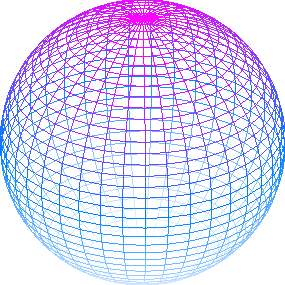
\includegraphics[scale=1]{../tikz/grad-math-tikz-pdf/sphere.pdf}
\end{minipage}\hfill
\begin{minipage}{.32\textwidth}\centering
	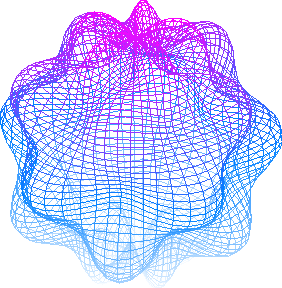
\includegraphics[scale=1]{../tikz/grad-math-tikz-pdf/sphere2.pdf}
\end{minipage}\hfill
\begin{minipage}{.32\textwidth}\centering
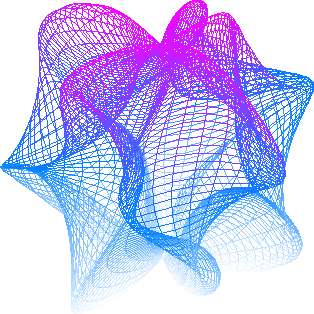
\includegraphics[scale=1]{../tikz/grad-math-tikz-pdf/sphere3.pdf}
\end{minipage}\hfill
\end{center}
\vfill
\begin{center}
\begin{minipage}{.32\textwidth}\centering
	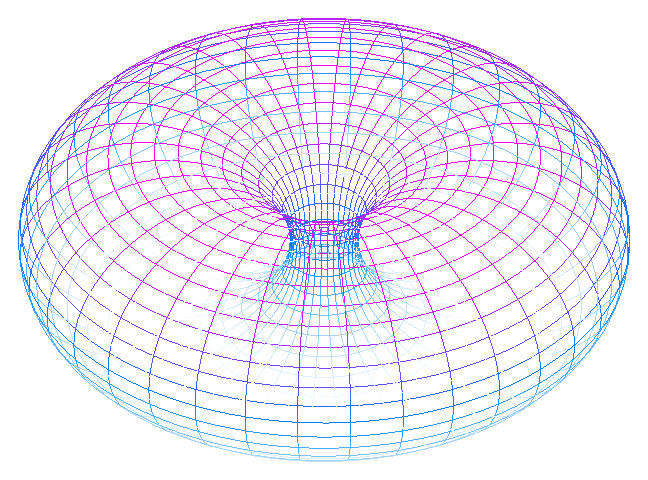
\includegraphics[scale=.525]{../tikz/grad-math-tikz-pdf/torus4.pdf}
\end{minipage}\hfill
\begin{minipage}{.32\textwidth}\centering
	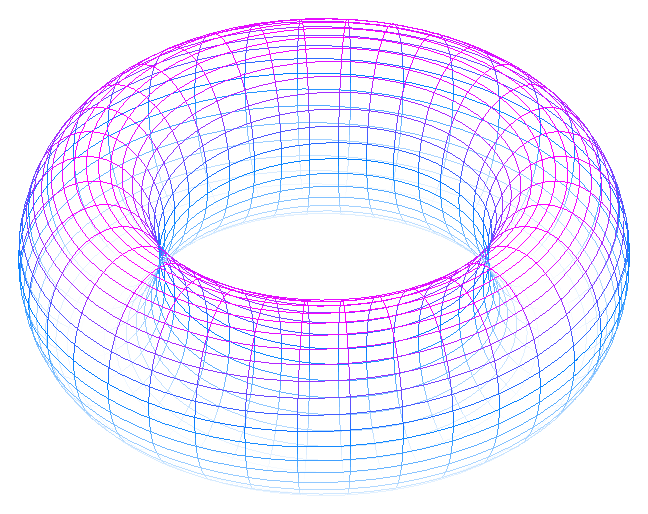
\includegraphics[scale=.525]{../tikz/grad-math-tikz-pdf/torus.pdf}
\end{minipage}\hfill
\begin{minipage}{.32\textwidth}\centering
	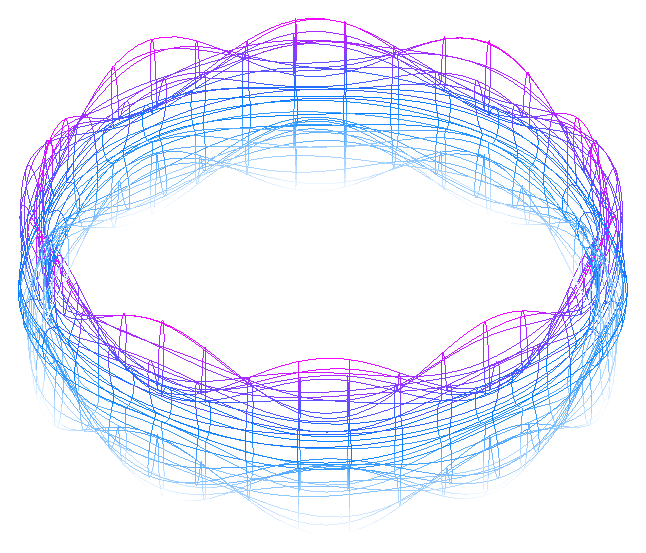
\includegraphics[scale=.525]{../tikz/grad-math-tikz-pdf/torus5.pdf}
\end{minipage}\hfill
\end{center}
\vfill
%\definecolor{mypurple}{HTML}{4C9FFF}
%\begin{center}
%\begin{tikzpicture}
%%	\def \x{3}
%%	\def \y{3.5}
%%	\draw[very thin,color=gray!15,step=.5] (-\x,-\y) grid (\x,\y);
%%	
%%	\foreach \i in {-\x,...,-2,-1,1,2,...,\x}
%%	\draw[gray] (\i,.1)--(\i,-.1) node[below] {$\i$};%x-axis
%%	\foreach \i in {-\y,-1,1,1,\y}
%%	\draw[gray] (.1,\i)--(-.1,\i) node[left] {$\i$};%y-axis
%	\begin{scope}[yshift=.5cm]
%	\node[mypurple] at (-4,2.75) {\LARGE\bf Length};
%	\draw[mypurple, line width=1mm] (-1,3) -- (1,3);
%	\draw[mypurple, line width=1mm] (-2,2.5) -- (2,2.5);
%	\end{scope}
%	\node[mypurple] at (-4,.5) {\LARGE\bf Area};
%	\filldraw[mypurple] (-2,0) rectangle (-1,1);
%	\filldraw[mypurple] (0,-1) rectangle (3,2);
%	\begin{scope}[yshift=-.5cm]	
%	\node[mypurple] at (-4,-2) {\LARGE\bf Angle};
%	\draw[mypurple, fill=mypurple, line width=.5mm] (-1.5,-1.5) -- (-2.5,-3) -- (-.5,-3) -- cycle;
%	\draw[mypurple, fill=mypurple, line width=.5mm] (.5,-3) -- (2.5,-3) -- (2.5, -1.5) -- cycle;
%	\end{scope}
%\end{tikzpicture}
%\end{center}

\newpage

\defbox[Topology; Topological Space]{\begin{definition*}
Let $S$ be a non-empty set. A \hl{\textbf{topology}}\footnote{The word ``topology'' comes from the Greek roots ``topos'' meaning ``place'' and ``logos'' meaning ``study''.} on $S$ is a subset $
\topology\subseteq 2^S$, where $2^S$ denotes the power set of $S$, that satisfies the following axioms: \begin{itemize}
	\item[(O1)\footnote{Empty set and Whole space}] The empty set and the entire set $S$ belong to $\topology$:\ $\boxed{S\in\topology\ \text{and}\ \varnothing\in\topology}$.
	\item[(O2)\footnote{Closure under \textit{arbitrary} unions}] The union of any collection of elements in $\topology$ is also an element of $\topology$: \[
	\boxed{\set{U_i}_{i\in I}\subseteq\topology\implies\bigcup_{i\in I}U_i\in\topology}.
	\]
	\item[(O3)\footnote{Closure under \textit{finite} intersections}] The intersection of any finite number of elements in $\topology$ is also an element of $\topology$: \[
	\boxed{\set{U_i}_{i=1}^n\subseteq\topology\implies\bigcap_{i=1}^n U_i\in\topology}.
	\]
\end{itemize}
The pair $(S,\topology)$ is called a \textbf{topological space}.
\end{definition*}}
\begin{remark*}
	By mathematical induction, we have \[
	\text{O3}\iff [\set{U_1,U_2}\subseteq\topology\Rightarrow U_1\cap U_2\in\topology].
	\]
\end{remark*}

%\begin{example}
%	Consider a set $S=\set{a,b,c,d,e}$. \begin{center}
%\begin{tikzpicture}[scale=.75]
%%	\def \x{3}
%%	\def \y{3}
%%	\draw[very thin,color=gray!15,step=.5] (-\x,-\y) grid (\x,\y);
%%	
%%	\foreach \i in {-\x,...,-2,-1,1,2,...,\x}
%%	\draw[gray] (\i,.1)--(\i,-.1) node[below] {$\i$};%x-axis
%%	\foreach \i in {-\y,-1,1,1,\y}
%%	\draw[gray] (.1,\i)--(-.1,\i) node[left] {$\i$};%y-axis
%	
%	\draw[rounded corners=8pt] (0, 3) -- (-1.5, 2.5) -- (-3, 1) -- (-2, .9) -- (-1.9, 0) -- (-2.5, -1) -- (-3, -2.5) -- (-2, -2) -- (0,-3) -- (2, -1.5) -- (3,-.5) -- (3,.5) -- (2, 1) -- (1.5, 1.5) -- (1.75, 2.5) -- cycle;
%	
%	\filldraw (0,1.5) circle (2pt) node[above] {$a$};
%	\filldraw (-1,.5) circle (2pt) node[above] {$c$};
%	\filldraw (1,0) circle (2pt) node[above] {$d$};
%	\filldraw (-.5,-2) circle (2pt) node[above] {$b$};
%	\filldraw (.5,-1) circle (2pt) node[above] {$e$};
%\end{tikzpicture}
%	\end{center}
%\begin{center}
%\begin{minipage}{.32\textwidth}
%\begin{tikzpicture}[scale=.75]
%%	\def \x{3}
%%	\def \y{3}
%%	\draw[very thin,color=gray!15,step=.5] (-\x,-\y) grid (\x,\y);
%%	
%%	\foreach \i in {-\x,...,-2,-1,1,2,...,\x}
%%	\draw[gray] (\i,.1)--(\i,-.1) node[below] {$\i$};%x-axis
%%	\foreach \i in {-\y,-1,1,1,\y}
%%	\draw[gray] (.1,\i)--(-.1,\i) node[left] {$\i$};%y-axis
%	
%	\draw[rounded corners=8pt] (0, 3) -- (-1.5, 2.5) -- (-3, 1) -- (-2, .9) -- (-1.9, 0) -- (-2.5, -1) -- (-3, -2.5) -- (-2, -2) -- (0,-3) -- (2, -1.5) -- (3,-.5) -- (3,.5) -- (2, 1) -- (1.5, 1.5) -- (1.75, 2.5) -- cycle;
%	
%	\filldraw (0,1.5) circle (2pt) node[above] {$a$};
%	\filldraw (-1,.5) circle (2pt) node[above] {$c$};
%	\filldraw (.5,0) circle (2pt) node[above] {$d$};
%	\filldraw (-.5,-1.5) circle (2pt) node[above] {$b$};
%	\filldraw (1,-1.5) circle (2pt) node[above] {$e$};
%	
%	\draw[line width=.5mm, opacity=.5, magenta] (0, 1.5) circle (10pt);
%	\draw[line width=.5mm, opacity=.5, orange, rotate=-20, xshift=-.15cm, yshift=.15cm] (0,0) ellipse (1.25cm and .5cm);
%	\draw[line width=.5mm, opacity=.5, green!50!black, yshift=.5cm] (0, 0) circle (40pt);
%	\draw[line width=.5mm, opacity=.5, cyan=-20, rotate=-20, xshift=0cm, yshift=-.5cm] (0,0) ellipse (1.75cm and 1.5cm);
%\end{tikzpicture}
%\end{minipage}
%\end{center}
%\end{example}
\vfill
\defbox[Open Set (Topology)]{\begin{definition*}
	Let $(S,\topology)$ be a topological space. $U\subseteq S$ is an \hl{\textbf{open set}}, or \textbf{open} (in $S$) iff $U\in\topology$.
\end{definition*}}
\begin{remark*}
A subset $\topology$ of power set $2^S$ is a topology on $S$ if and only if \begin{enumerate}
	\item[(i)] $\varnothing$ and $S$ are open;
	\item[(ii)] Let $U_1,U_2,\dots\in\topology$, \ie, $\set{U_i}_{i\in I}\subseteq\topology$. Then $\displaystyle\bigcup_{i\in I}U_i$ is open.
	\item[(iii)] Let $U_1,U_2,\dots, U_n\in\topology$, \ie, $\set{U_i}_{i=1}^n\subseteq\topology$. Then $\displaystyle\bigcap_{i=1}^n U_i$ is open.
\end{enumerate}
\end{remark*}
\defbox[Continuous Mapping by Open Sets]{\begin{definition*}
	Let $(X,\topology_X)$ and $(Y,\topology_Y)$ are topological spaces. Let $f:X\to Y$ be a mapping from $X$ to $Y$. \begin{enumerate}[(1)]
%		\item (Continuous at a Point) Let $x\in X$. The mapping $f$ is \textbf{continuous at} $\boldsymbol{x}$ if and only if \[
%		\forall U_Y\in\topology_Y,f(x)\in U_Y,\ \exists U_X\in\topology_X\ \text{such that}\ x\in U_X\land f[U_X]\subseteq U_Y.
%		\]
%		\item (Continuous on a Set) Let $S\subseteq X$. The mapping $f$ is \textbf{continuous on} $\boldsymbol{S}$ if and only if $f$ is continuous at every point $x\in S$.
		\item (Continuous Everywhere) The mapping $f$ is \textbf{continuous on} $\boldsymbol{X}$ if and only if \[
		U_Y\in\topology_Y\implies f^{-1}[U_Y]\in\topology_X,
		\] where $f^{-1}[U_Y]=\set{x\in X:f(x)\in U_Y}$ is the preimage of $U_Y$ under $f$.
		\begin{center}\adjustbox{scale=.95}{
		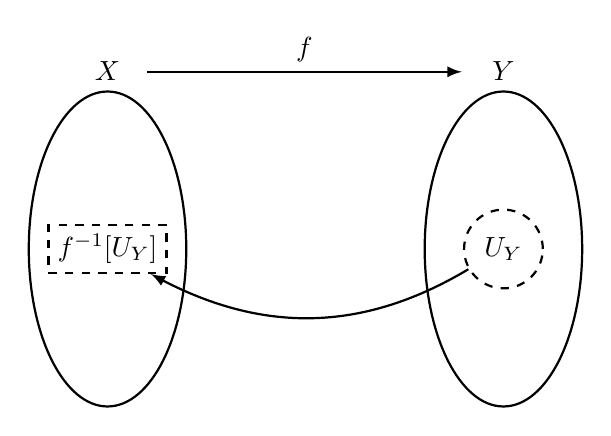
\begin{tikzpicture}[thick] 
			\node[ellipse,draw,minimum width=2cm,minimum height=4cm,label=above:$X$] (X) {};
			\node[ellipse,draw,minimum width=2cm,minimum height=4cm,right=3cm of X,label=above:$Y$]
			(Y){};
			\node[dashed,draw] (f) at (X.center) {$f^{-1}[U_Y]$};
			\node[circle,dashed,draw,minimum size=1cm] (U) at (Y.center) {$U_Y$};
			\draw[-latex] (0.5,2.25) -- (4.5,2.25) node[midway,above]{$f$};
			\draw[-latex] (U) to[bend left] (f);
		\end{tikzpicture}}
		\end{center}
	\end{enumerate}
\end{definition*}}
\vfill
\begin{note}[Preparation for \textbf{Example 1}]
	Let $S\neq\varnothing$ be a set, and let $\set{A_\alpha}_{\alpha\in\Lambda}\subseteq S$. Then
	\begin{align*}
		S\setminus\bigcup_{\alpha\in\Lambda}A_\alpha=S\setminus\set{x\in S:\exists \alpha\in\Lambda\ \text{s.t.}\ x\in A_\alpha}
		&=\set{x\in S:\lnot [\exists \alpha\in\Lambda\ \text{s.t.}\ x\in A_\alpha]}\\
		&=\set{x\in S:\forall \alpha\in\Lambda,\ x\notin A_\alpha}\\
		&=\set{x\in S:\forall \alpha\in\Lambda,\ x\in S\setminus A_\alpha}\\
		&=\bigcap_{\alpha\in\Lambda}(S\setminus A_\alpha).
	\end{align*}
	\begin{align*}
		S\setminus\bigcap_{\alpha\in\Lambda}A_\alpha=S\setminus\set{x\in S:\forall\alpha\in\Lambda,\ x\in A_\alpha}
		&=\set{x\in S:\lnot [\forall\alpha\in\Lambda,\ x\in A_\alpha]}\\
		&=\set{x\in S:\exists \alpha\in\Lambda\ \text{s.t.}\ x\notin A_\alpha}\\
		&=\set{x\in S:\exists \alpha\in\Lambda\ \text{s.t.}\ x\in S\setminus A_\alpha}\\
		&=\bigcup_{\alpha\in\Lambda}(S\setminus A_\alpha).
	\end{align*}
\end{note}
\vfill
\begin{note}[Preparation for \textbf{Example 1}]
\ \begin{enumerate}[(1)]
	\item A Subset of a Finite Set is Finite.
	\item The Intersection of Finite Sets is Finite.
\end{enumerate}
\end{note}
\vfill
\begin{example}[Cofinite Topology]
	Let $S\neq\varnothing$ be a set. Define the cofinite topology $\topology_C\subseteq 2^S$ by \begin{align*}
	\topology_C:&=\set{U\subseteq S:S\setminus U\ \text{is finite}}\cup\set{\varnothing}\\
	&=\set{U\subseteq S:U=\varnothing\ \text{or}\ S\setminus U\ \text{is finite}}.
	\end{align*} In other words, $U$ is open in the cofinite topology if $U$ is the empty, or if the complement $S\setminus U$ is a finite set. We claim that $\topology_C$ be a topology on $S$:
	\begin{enumerate}[(O1)]
		\item By definition, $\varnothing\in\topology_C$. For $U=S$, the complement $S\setminus S=\varnothing$, which is finite, so $S\in\topology_C$. Hence, both $\varnothing$ and $S$ are elements of $\topology_C$.
		\item Let $\set{U_i}_{i\in I}\subseteq\topology_C$. 
		\begin{itemize}
			\item[(Case 1)] If $U_i=\varnothing$ for all $i\in I$, then $\bigcup_{i\in I}U_i=\varnothing\in\topology_C$. 
			\item[(Case 2)] Suppose that there exists $i_0\in I$ such that $U_{i_0}\neq\varnothing$. Then \[
			S\setminus\bigcup_{i\in I}U_i=\bigcap_{i\in I}\left(S\setminus U_i\right)\subseteq (S\setminus U_{i_0}).
			\]
			Since $S\setminus U_{i_0}$ is finite, $S\setminus\bigcup_{i\in I}U_i$ if finite, so $\bigcup_{i\in I} U_i\in\topology_C$.
		\end{itemize}
		\item Let $U_1\in\topology_C$ and $U_2\in\topology_C$. 
		\begin{itemize}
			\item[(Case 1)] If $U_1=\varnothing$ or $U_2=\varnothing$, then $U_1\cap U_2=\varnothing\in\topology_C$. 
			\item[(Case 2)] Suppose that $U_1\neq\varnothing$ and $U_2\neq\varnothing$. Then $S\setminus U_1$ and $S\setminus U_2$ are finite. By the De Morgan law, we have \[
			S\setminus(U_1\cap U_2)=(S\setminus U_1)\cup (S\setminus U_2),
			\] which is a finite set. Thus, $U_1\cap U_2\in\topology_C$.
		\end{itemize}
	\end{enumerate}
\end{example}

\newpage
\begin{example}[Discrete Topology]
	Let $S\neq\varnothing$ be a set, and let $\topology=2^S$ be the power set of $S$. Then $\topology$ is called the \textbf{discrete topology} on $S$ and $(S,\topology)=(S,2^S)$ the \textbf{discrete (topological) space} on $S$.
\end{example}
\vfill
\begin{example}[Indiscrete Topology]
	Let $S\neq\varnothing$ be a set, and let $\topology=\set{S,\varnothing}$. Then $\topology$ is called the \textbf{indiscrete topology} on $S$ and $(S,\topology)=(S,\set{S,\varnothing})$ the \textbf{indiscrete (topological) space} on $S$.
\end{example}
\vfill
\begin{note}
\ \begin{enumerate}[(1)]
	\item Discrete Topology is Finest Topology.
	\item Indiscrete Topology is Coarsest Topology.
\end{enumerate}
\end{note}
\vfill
\defbox[Coarser Topology and Finer Topology]{\begin{definition*}
	Let $S\neq\varnothing$ be a set. Let $\topology_1$ and $\topology_2$ be topologies on $S$.
	\begin{enumerate}[(1)]
		\item $\topology_1$ is said to be \textbf{coarser} than $\topology_2$ if $\topology_1\subseteq \topology_2$.
		\item $\topology_1$ is said to be \textbf{finer} than $\topology_2$ if $\topology_2\subseteq \topology_1$.
	\end{enumerate}
\end{definition*}}
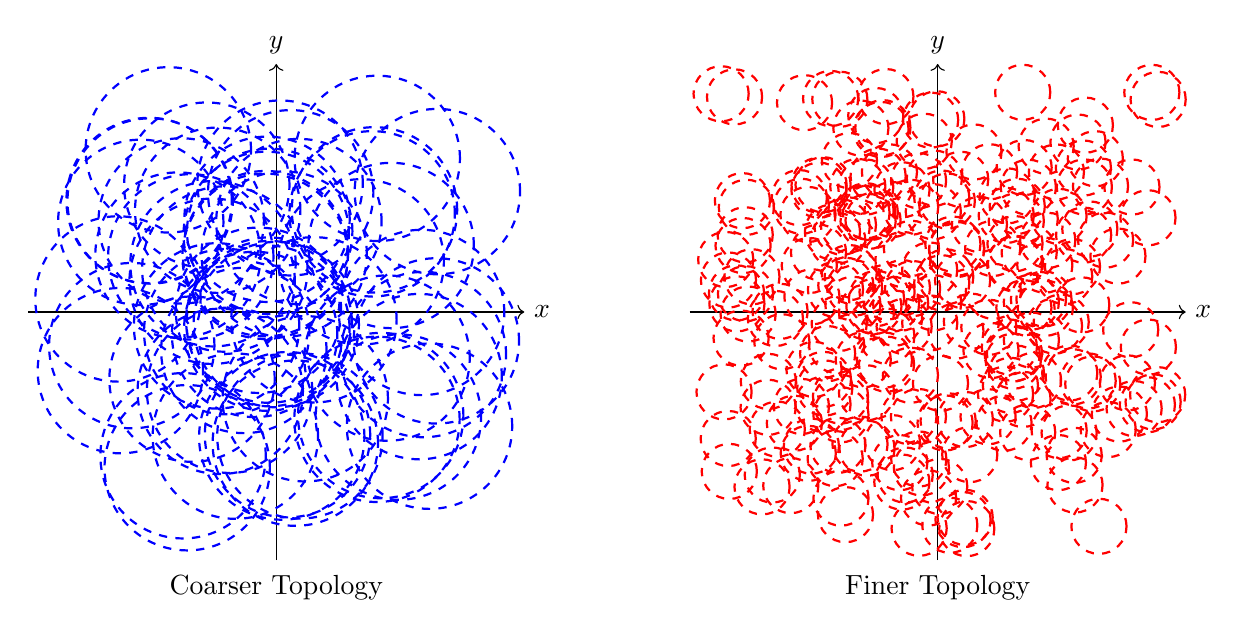
\begin{tikzpicture}[scale=.7]
	
	% Coarser Topology on the left
	\begin{scope}[shift={(-6,0)}]
		% Axes
		\draw[->] (-4.5,0) -- (4.5,0) node[right] {$x$};
		\draw[->] (0,-4.5) -- (0,4.5) node[above] {$y$};
		\node at (0,-5) {Coarser Topology};
		
		% Randomly placed large dashed open balls using modular arithmetic
		\foreach \i in {1,2,...,20} {
			\pgfmathsetmacro{\randx}{rand*3.3} % Random value
			\pgfmathsetmacro{\randy}{rand*3.3} % Random value
			\pgfmathsetmacro{\x}{mod(\randx, 3)} % Map to [-4, 4]
			\pgfmathsetmacro{\y}{mod(\randy, 3)} % Map to [-4, 4]
			\pgfmathsetmacro{\r}{1.5} % Random radius between 1.5 and 2.5
			\draw[blue, dashed, thick] (\x,\y) circle (\r);
		}
		\foreach \i in {1,2,...,20} {
			\pgfmathsetmacro{\randx}{rand*3.3} % Random value
			\pgfmathsetmacro{\randy}{rand*3.3} % Random value
			\pgfmathsetmacro{\x}{mod(\randx, 3)} % Map to [-4, 4]
			\pgfmathsetmacro{\y}{mod(\randy, 3)} % Map to [-4, 4]
			\pgfmathsetmacro{\r}{1.5} % Random radius between 1.5 and 2.5
			\draw[blue, dashed, thick] (\x,\y) circle (\r);
		}
		\foreach \i in {1,2,...,20} {
			\pgfmathsetmacro{\randx}{rand*3.3} % Random value
			\pgfmathsetmacro{\randy}{rand*3.3} % Random value
			\pgfmathsetmacro{\x}{mod(\randx, 3)} % Map to [-4, 4]
			\pgfmathsetmacro{\y}{mod(\randy, 3)} % Map to [-4, 4]
			\pgfmathsetmacro{\r}{1.5} % Random radius between 1.5 and 2.5
			\draw[blue, dashed, thick] (\x,\y) circle (\r);
		}
	\end{scope}
	
	% Finer Topology on the right
	\begin{scope}[shift={(6,0)}]
		% Axes
		\draw[->] (-4.5,0) -- (4.5,0) node[right] {$x$};
		\draw[->] (0,-4.5) -- (0,4.5) node[above] {$y$};
		\node at (0,-5) {Finer Topology};
		
		% Randomly placed smaller dashed open balls using modular arithmetic
		\foreach \i in {1,2,...,75} {
			\pgfmathsetmacro{\randx}{rand*6.5} % Random value
			\pgfmathsetmacro{\randy}{rand*6.5} % Random value
			\pgfmathsetmacro{\x}{mod(\randx, 4)} % Map to [-4, 4]
			\pgfmathsetmacro{\y}{mod(\randy, 4)} % Map to [-4, 4]
			\pgfmathsetmacro{\r}{0.5} % Random radius between 0.5 and 1
			\draw[red, dashed, thick] (\x,\y) circle (\r);
		}
		\foreach \i in {1,2,...,75} {
			\pgfmathsetmacro{\randx}{rand*6.5} % Random value
			\pgfmathsetmacro{\randy}{rand*6.5} % Random value
			\pgfmathsetmacro{\x}{mod(\randx, 4)} % Map to [-4, 4]
			\pgfmathsetmacro{\y}{mod(\randy, 4)} % Map to [-4, 4]
			\pgfmathsetmacro{\r}{0.5} % Random radius between 0.5 and 1
			\draw[red, dashed, thick] (\x,\y) circle (\r);
		}
		\foreach \i in {1,2,...,75} {
			\pgfmathsetmacro{\randx}{rand*6.5} % Random value
			\pgfmathsetmacro{\randy}{rand*6.5} % Random value
			\pgfmathsetmacro{\x}{mod(\randx, 4)} % Map to [-4, 4]
			\pgfmathsetmacro{\y}{mod(\randy, 4)} % Map to [-4, 4]
			\pgfmathsetmacro{\r}{0.5} % Random radius between 0.5 and 1
			\draw[red, dashed, thick] (\x,\y) circle (\r);
		}
	\end{scope}
\end{tikzpicture}
%\begin{tikzpicture}[scale=1.5]
%	
%	% Coarser Topology
%	\draw[thick] (-3,0) circle (1.5) node[above=1.7cm, align=center] {Coarser Topology\\(Fewer Open Sets)};
%	\draw[thick, dashed, blue] (-3,0) circle (1);
%	\draw[thick, dashed, red] (-3,0) circle (0.5);
%	
%	% Finer Topology
%	\draw[thick] (3,0) circle (1.5) node[above=1.7cm, align=center] {Finer Topology\\(More Open Sets)};
%	\draw[thick, dashed, blue] (3,0) circle (1.25);
%	\draw[thick, dashed, red] (3,0) circle (1);
%	\draw[thick, dashed, green] (3,0) circle (0.75);
%	\draw[thick, dashed, orange] (3,0) circle (0.5);
%	\draw[thick, dashed, purple] (3,0) circle (0.25);
%	
%	% Annotations
%%	\node[below=2cm, align=center] at (0,-2.2) {Visualization: Coarser topologies have larger,\\ less refined open sets. Finer topologies\\ have smaller, more nested open sets.};
%	
%	% Arrow between topologies
%%	\draw[thick, ->, >=stealth] (-1.2,0) -- (1.2,0) node[midway, above] {Finer};
%	
%\end{tikzpicture}

%\begin{tikzpicture}[scale=.7]
%	
%	% Coarser Topology on the left
%	\begin{scope}[shift={(-6,0)}]
%		% Axes
%		\draw[->] (-4,0) -- (4,0) node[right] {$x$};
%		\draw[->] (0,-4) -- (0,4) node[above] {$y$};
%		\node at (0,-4.5) {Coarser Topology};
%		
%		% Large dashed open balls covering the entire space
%		\foreach \x in {-3, 0, 3} {
%			\foreach \y in {-3, 0, 3} {
%				\draw[blue, dashed, thick] (\x,\y) circle (2);
%			}
%		}
%	\end{scope}
%	
%	% Finer Topology on the right
%	\begin{scope}[shift={(6,0)}]
%		% Axes
%		\draw[->] (-4,0) -- (4,0) node[right] {$x$};
%		\draw[->] (0,-4) -- (0,4) node[above] {$y$};
%		\node at (0,-4.5) {Finer Topology};
%		
%		% Smaller dashed open balls covering the entire space
%		\foreach \x in {-3, -2, -1, 0, 1, 2, 3} {
%			\foreach \y in {-3, -2, -1, 0, 1, 2, 3} {
%				\draw[red, dashed, thick] (\x,\y) circle (0.8);
%			}
%		}
%	\end{scope}
%	
%\end{tikzpicture}
%\begin{tikzpicture}[scale=1]
%	
%	% Coarser Topology
%	\node at (-4.5, 3.2) {\textbf{Coarser Topology}};
%	\draw[thick, blue] (-6, 3) -- (-3, 3); % Entire real line representation
%	\node at (-4.5, 2.8) {\(\mathbb{R}\) (entire space)};
%	\draw[thick, blue, dashed] (-6, 2) -- (-4.5, 2) -- (-4.5, 2.3); % (-∞, 0)
%	\node[blue] at (-5.5, 1.8) {\((- \infty, 0)\)};
%	\draw[thick, blue] (-4.5, 2) -- (-3, 2); % [0, ∞)
%	\node[blue] at (-3.5, 1.8) {\([0, \infty)\)};
%	
%	% Finer Topology
%	\node at (4.5, 3.2) {\textbf{Finer Topology}};
%	\draw[thick, red] (2, 3) -- (7, 3); % Entire real line representation
%	\node at (4.5, 2.8) {\(\mathbb{R}\)};
%	\draw[thick, red] (3.5, 2) -- (5.5, 2); % Interval (0, 2)
%	\node[red] at (4.5, 1.8) {\((0, 2)\)};
%	\draw[thick, red] (2.8, 1) -- (6.2, 1); % Interval (-1, 1)
%	\node[red] at (4.5, 0.8) {\((-1, 1)\)};
%	
%	% Labels
%	\node at (-4.5, 1) {\textbf{Fewer Open Sets}};
%	\node at (4.5, 0) {\textbf{More Open Sets}};
%	
%	% Arrows to show refinement
%	\draw[->, thick] (-1, 2) -- (1, 2) node[midway, above] {\textit{Refinement}};
%	\draw[->, thick] (1, 1) -- (-1, 1) node[midway, below] {\textit{Coarsening}};
%	
%\end{tikzpicture}
%\begin{tikzpicture}[scale=1.5]
%	
%	% Coarser Topology
%	\node at (-3, 2.5) {\textbf{Coarser Topology}};
%	\draw[thick, blue] (-4, 1) rectangle (-2, 3);
%	\draw[thick, dashed, blue] (-4.5, 0.5) rectangle (-1.5, 3.5);
%	
%	% Labels for Coarser Topology
%	\node[blue] at (-4.5, 0.2) {\small Larger Open Sets};
%	\node[blue] at (-3, 3.3) {\small Fewer Subsets};
%	
%	% Finer Topology
%	\node at (3, 2.5) {\textbf{Finer Topology}};
%	\draw[thick, red] (1, 1) rectangle (3, 3);
%	\draw[thick, dashed, red] (0.5, 0.5) rectangle (3.5, 3.5);
%	
%	% Subdivisions within Finer Topology
%	\draw[thick, red] (2, 1) -- (2, 3); % Vertical division
%	\draw[thick, red] (1, 2) -- (3, 2); % Horizontal division
%	
%	% Labels for Finer Topology
%	\node[red] at (0.5, 0.2) {\small More Open Sets};
%	\node[red] at (3, 3.3) {\small More Subsets};
%	
%	% Arrows showing finer to coarser
%	\draw[->, thick] (-1, 2) -- (1, 2) node[midway, above] {\textit{Refinement}};
%	\draw[->, thick] (1, 1) -- (-1, 1) node[midway, below] {\textit{Coarsening}};
%	
%\end{tikzpicture}
\vfill
\newpage
\defbox[Distance Function]{\begin{definition*}
	Let $S$ be a set. The real-valued function of two variable \[
	d:S\times S\to\R
	\] is called a \textbf{distance function} (or \hl{\textbf{metric}}) if it satisfies the following properties:
	\begin{enumerate}[(i)]
		\item[(i)\footnote{Non-negativity and Zero only for identical points}]$\forall x,y\in S,\ d(x,y)\geq 0\quad\text{and}\quad d(x,y)=0\Leftrightarrow x=y.$
		\item[(ii)\footnote{Symmetry}] $\forall x,y\in S,\ d(x,y)=d(y,x).$
		\item[(iii)\footnote{Triangle inequality}] $\forall x,y,z\in S,\ d(x,z)\leq d(x,y)+d(y,z).$
	\end{enumerate} The pair $(S,d)$ is called a \textbf{metric space}.
\end{definition*}}
\begin{remark*}
\ \begin{center}
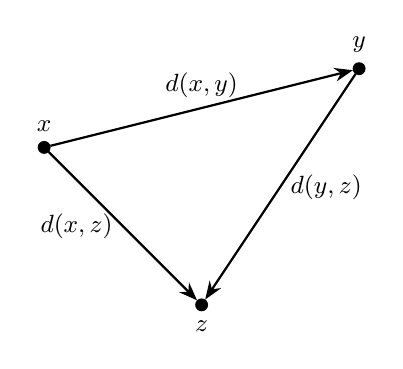
\begin{tikzpicture}[>=Stealth, scale=2, every node/.style={font=\small}]
	% Points in the space
	\node[draw, circle, fill=black, inner sep=1.5pt, label=above:$x$] (x) at (0, 0) {};
	\node[draw, circle, fill=black, inner sep=1.5pt, label=above:$y$] (y) at (2, 0.5) {};
	\node[draw, circle, fill=black, inner sep=1.5pt, label=below:$z$] (z) at (1, -1) {};
	
	% Edges for distances
	\draw[->, thick] (x) -- (y) node[midway, above] {$d(x,y)$};
	\draw[->, thick] (y) -- (z) node[midway, right] {$d(y,z)$};
	\draw[->, thick] (x) -- (z) node[midway, left] {$d(x,z)$};
	
%	% Non-negativity and zero for identical points
%	\node at (0, -1.5) [text width=5cm, align=center] 
%	{\footnotesize (i) Non-negativity: $d(x,y) \geq 0$ \\
%		Zero if $x=y$: $d(x,y) = 0 \Leftrightarrow x = y$};
%	
%	% Symmetry illustration
%	\draw[<->, dashed, thick, color=blue] (0.5, 0.25) arc[start angle=30, end angle=180, radius=0.5];
%	\draw[<->, dashed, thick, color=blue] (1.5, 0.25) arc[start angle=150, end angle=330, radius=0.5];
%	\node[blue] at (1, 0.8) {\footnotesize (ii) Symmetry: $d(x,y) = d(y,x)$};
%	
%	% Triangle inequality illustration
%	\draw[dotted, thick, color=red] (0.5, 0) -- (1.5, -0.25);
%	\node[red, align=center] at (1.5, -0.7) 
%	{\footnotesize (iii) Triangle inequality: \\ $d(x,z) \leq d(x,y) + d(y,z)$};
%	
%	% Optional labels for the set
%	\node at (-0.3, 0) {\small $S$};
%	\draw[rounded corners, dashed] (-1, -1.5) rectangle (2.5, 1.5) {};
	
\end{tikzpicture}
\end{center}
\end{remark*}
\begin{example}
\ \begin{itemize}
	\item Let $S=\R$, the set of real numbers. Define the function $d:\R\times\R\to\R$ by \[d(x,y)=\abs{x-y}\] for $x,y\in\R$.
	\item Let $S=\R^n$, the $n$-dimensional Euclidean space. Define the function $d:\R^n\times\R^n\to\R$ by \[
	d(\textbf{x},\textbf{y})=\norm{\textbf{x}-\textbf{y}}=\sqrt{\sum_{i=0}^{n-1}\abs{x_i-y_i}^2},
	\] where $\textbf{x}=(x_0,x_1,\dots x_{n-1})$ and $\textbf{y}=(y_0,\dots, y_{n-1})$ are vectors in $\R^n$.
\end{itemize}
\end{example}
\newpage
\defbox[Neighborhood (Metric Space)]{\begin{definition*}
 Let $(S,d)$ be a metric space, where $S$ is a set and $d:S\times S\to\R$ is a metric. For $x\in S$ and $\varepsilon>0$, the \hl{\textbf{$\boldsymbol{\varepsilon}$-neighborhood of $x$}} , denoted by $\nbhd_\varepsilon(x)$, is defined as \[
 \nbhd_\varepsilon(x):=\set{y\in S:d(x,y)<\varepsilon}.
 \]
\end{definition*}}
\begin{remark*}
\ \begin{center}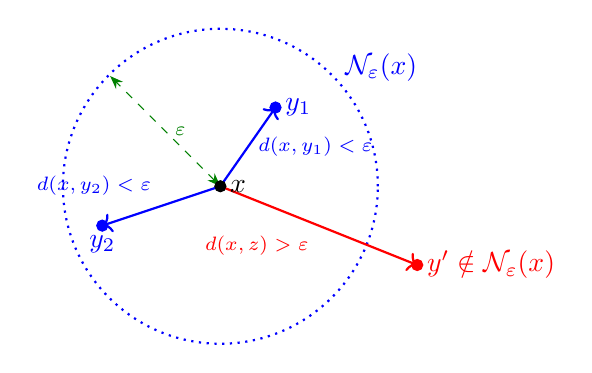
\begin{tikzpicture}[scale=1]
	% Draw the main set S as a large circle
%	\draw[thick, dashed, gray] (0,0) circle [radius=3] node[below left=3cm, black] {Set $S$};
	
	% Draw the epsilon-neighborhood
	\draw[dotted, thick, blue] (0,0) circle [radius=2];
	\node[above right=0.3cm] at (1.25,1) {\textcolor{blue}{$\nbhd_\varepsilon(x)$}};
	
	% Add some sample points within the epsilon-neighborhood
	\filldraw[blue] (0.7,1) circle (2pt) node[right] {$y_1$};
	\filldraw[blue] (-1.5,-.5) circle (2pt) node[below] {$y_2$};
	
	% Add a sample point outside the epsilon-neighborhood
	\filldraw[red] (2.5,-1) circle (2pt) node[right] {$y'\notin\nbhd_\varepsilon(x)$};
	
	% Add arrows to indicate distances
	\draw[>=Stealth, <->, dashed, green!50!black] (0,0) -- (-1.4,1.4) node[midway, right] {\scriptsize $\varepsilon$};
	\draw[blue, ->, thick] (0,0) -- (0.7,1) node[midway, right] {\scriptsize $d(x,y_1)<\varepsilon$};
	\draw[blue, ->, thick] (0,0) -- (-1.5,-.5) node[midway, above left] {\scriptsize $d(x,y_2)<\varepsilon$};
	\draw[red, ->, thick, red] (0,0) -- (2.5,-1) node[midway, below left] {\scriptsize \textcolor{red}{$d(x,z)>\varepsilon$}};
	
	% Mark the point x
	\filldraw[black] (0,0) circle (2pt) node[right] {$x$};
\end{tikzpicture}\end{center}
\end{remark*}

\defbox[Open Set (Metric Space)]{\begin{definition*}
	Let $(S,d)$ be a metric space, where $S$ is a set and $d:S\times S\to\R$ is a metric.
 	Then
%	$U$ is an \textbf{open set} in $S$ (as metric space) if and only if 
	\[
	U\subseteq S\ \text{is \textbf{open} in}\ S\overset{\textnormal{def}}{\iff}\forall p\in U,\ \exists\varepsilon>0\ \text{such that}\ \nbhd_\varepsilon(p)\subseteq U.
	\]
\end{definition*}}
\begin{remark*}
\ \begin{center}
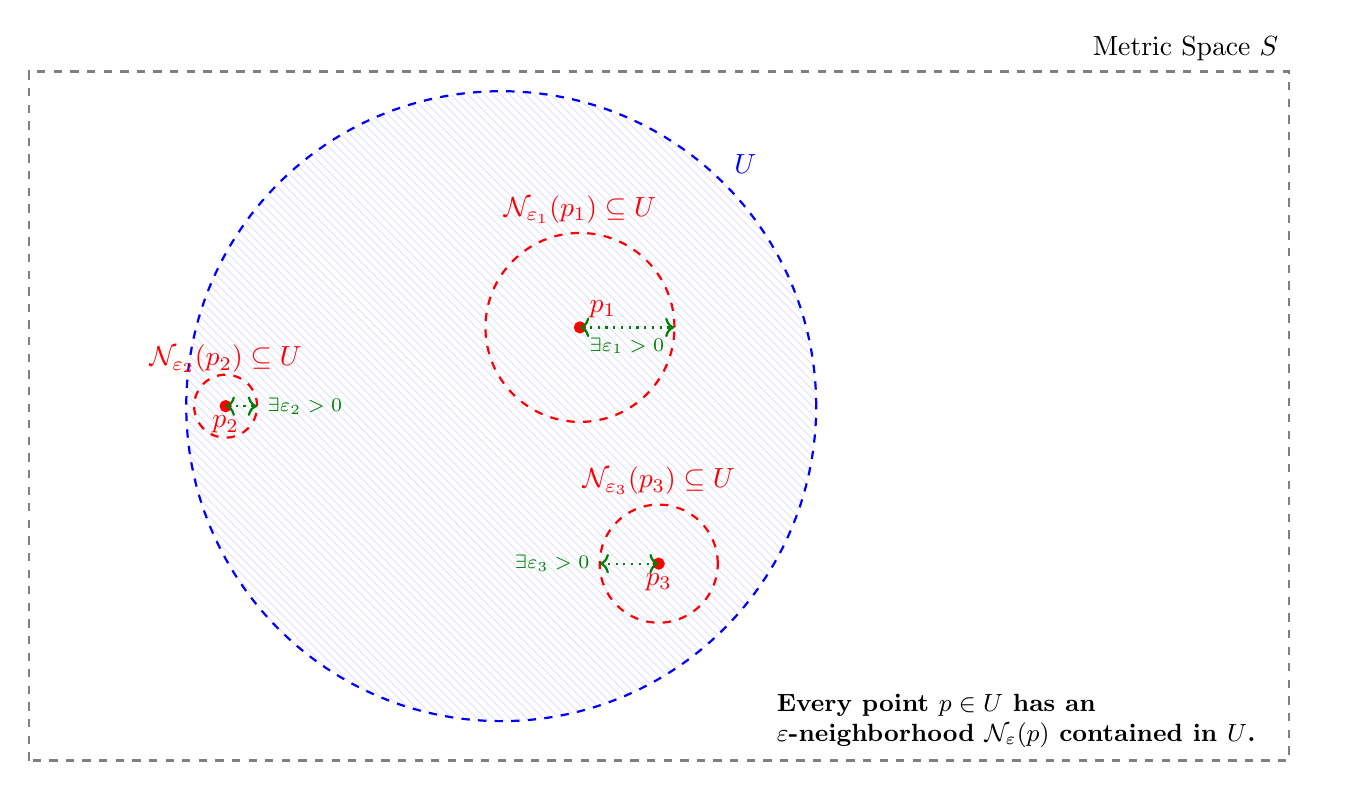
\begin{tikzpicture}[scale=1]
	% Draw the main set S
	\draw[thick, dashed, gray] (-6,-4.5) rectangle (10,4.25) node[black, above left] {Metric Space $S$};
%	\draw[thick, dashed, gray] (0,0) circle [radius=5] node[above right=4cm, black] {Metric Space $S$};
	
	% Draw the subset U
%	\fill[blue!10] (0,0) circle [radius=4];
	\fill[pattern=north west lines, pattern color=blue!10] (0,0) circle [radius=4];
	\draw[dashed, thick, blue] (0,0) circle [radius=4] node[above right=4cm, blue] {$U$};
	
	% Mark a point p in U
	\filldraw[red] (1,1) circle (2pt) node[above right] {$p_1$};
	\filldraw[red] (-3.5,0) circle (2pt) node[below] {$p_2$};
	\filldraw[red] (2,-2) circle (2pt) node[below] {$p_3$};
	
	% Draw the epsilon-neighborhood around p
	\draw[dashed, thick, red] (1,1) circle [radius=1.2];
	\node[above=1.2cm] at (1,1) {\textcolor{red}{ $\nbhd_{\varepsilon_1}(p_1)\subseteq U$}};
	\draw[<->, dotted, thick, green!50!black] (1,1) to (2.2,1) node[below left] {\scriptsize $\exists\varepsilon_1>0$};
	
	\draw[dashed, thick, red] (-3.5,0) circle [radius=.4];
	\node[above=0.3cm] at (-3.5,0) {\textcolor{red}{$\nbhd_{\varepsilon_2}(p_2)\subseteq U$}};
	\draw[<->, dotted, thick, green!50!black] (-3.5,0) to (-3.1,0) node[right] {\scriptsize $\exists\varepsilon_2>0$};
	
	\draw[dashed, thick, red] (2,-2) circle [radius=.75];
	\node[above=0.75cm] at (2,-2) {\textcolor{red}{$\nbhd_{\varepsilon_3}(p_3)\subseteq U$}};
	\draw[<->, dotted, thick, green!50!black] (2,-2) to (1.25,-2) node[left] {\scriptsize $\exists\varepsilon_3>0$};
	
	% Add a sample point inside the epsilon-neighborhood
%	\filldraw[black] (1.8,1.5) circle (2pt) node[right] {$q \in \nbhd_\varepsilon(p)$};
	
	% Add text labels
	\node[] at (7,-4) {
		\begin{minipage}{7cm}
			\small
			\textbf{Every point $p \in U$ has an}\\ \textbf{$\varepsilon$-neighborhood $\nbhd_\varepsilon(p)$ contained in $U$.}
		\end{minipage}
	};
	% Arrow showing that epsilon-neighborhood is within U
%	\draw[->, thick, blue] (2.5,0.5) -- (1.2,1) node[midway, above, blue] {$\nbhd_\varepsilon(p) \subseteq U$};
\end{tikzpicture}
\end{center}
\end{remark*}
\newpage
\begin{exercise*}[Metric Topology]
	Let $(S,d)$ be a metric space, where $S$ is a set and $d:S\times S\to\R$ is a metric. Consider the set $\tau$ of all open sets of $S$: \begin{align*}
	\tau:&=\set{U\subseteq S:U\ \text{is open in}\ S} \\
	&=\set{U\subseteq S:\forall p\in U,\ \exists\varepsilon>0\ \text{such that}\ \nbhd_\varepsilon(p)\subseteq U}.
	\end{align*} We claim that $\tau$ is the topology induced by the metric $d$ on the space $S$: \begin{enumerate}[(\text{O}1)]
	\item $S\in\tau$ and $\varnothing\in\tau$:
	
	($\varnothing\in\tau$)\ The condition \begin{center}
		``$\forall p\in U,\ \exists\varepsilon>0\ \text{such that}\ \nbhd_\varepsilon(p)\subseteq U$''
	\end{center} is vacuously true for $U=\varnothing$. Therefore $\varnothing\in\tau$.
	
	($S\in\tau$)\ For $p\in S$, the $\varepsilon$-neighborhhod of $p$ is defined as\[
	\nbhd_\varepsilon(p)=\set{q\in S: d(p,q)<\varepsilon}\subseteq S.
	\] Since $S$ is the entire space, $\nbhd_\varepsilon(p)\subseteq S$ for any 
	$\varepsilon>0$.
	\item $\tau$ is closed under arbitrary unions:
	
	Let $\set{U_i}_{i\in I}$ be an arbitrary collection of sets in $\tau$. Let $p\in\bigcup_{i\in I}U_i$. Then \[
	\exists i_0\in I\quad\text{such that}\quad p\in U_{i_0}.
	\] Since $U_{i_0}\in\tau$, there exists $\varepsilon>0$ such that $\nbhd_\epsilon(p)\subseteq U_{i_0}$. Then \[
	\nbhd_\epsilon(p)\subseteq U_{i_0}\subseteq\bigcup_{i\in I}U_i.
	\] Thus, $\bigcup_{i\in I}U_i\in\tau$.
	\item $\tau$ is closed under finite intersections:
	
	Let $U_1,U_2\in\tau$, and let $p\in (U_1\cap U_2)$. Then \begin{align*}
		\exists\varepsilon_1>0\quad\text{such that}\quad \nbhd_{\varepsilon_1}(p)\subseteq U_1,\\
		\exists\varepsilon_2>0\quad\text{such that}\quad \nbhd_{\varepsilon_2}(p)\subseteq U_2.
	\end{align*} Define $\varepsilon:=\min(\varepsilon_1,\varepsilon_2)$. Then \[
		\nbhd_\varepsilon(p)\subseteq\nbhd_{\varepsilon_i}(p)\subseteq U_i\quad\text{for }\quad i=1,2.
	\] Thus $\nbhd_{\varepsilon}(p)\subset U_1\cap U_2$, and so $U_1\cap U_2\in\tau$.
\end{enumerate}
\end{exercise*}

\begin{note}[Convergence of Sequences]
	A sequence $\set{a_n}_{n=1}^\infty(\subseteq\R)$ is \textbf{converge} to $L\in\R$ if and only if 
	\begin{align*}
	&\forall\varepsilon>0,\ \exists N\in\N\ \text{such that}\ \left[ n\geq N\implies \abs{a_n-L}<\varepsilon\right]\\
	\iff&\forall\varepsilon>0,\ \exists N\in\N\ \text{such that}\ \left[ n\geq N\implies d(a_n,L)<\varepsilon\right]\\
	\iff&\forall\varepsilon>0,\ \exists N\in\N\ \text{such that}\ \left[ n\geq N\implies a_n\in\nbhd_\varepsilon (L)\right]
	\end{align*}
\begin{center}
\begin{tikzpicture}[scale=.6]
	% Define the coordinates for L and the bounding lines
	\def\L{3} % Set L at 3 for visualization
	\def\epsilon{1} % Epsilon value
	\def\N{14} % Example N value
	\def\xMax{25}
	\def\yMax{6} % Max value for y-axis
	
	% Draw axes
	\draw[thick,-Stealth] (0,0) -- (\xMax+1,0) node[anchor=west] {$n$};
	\draw[thick,-Stealth] (0,0) -- (0,\yMax) node[anchor=south] {$a_n$};
	
	% Draw L and epsilon lines
	\draw[dashed, magenta, opacity=.3] (0,\L) -- (\xMax+1,\L) node[right] {$L$};
	\draw[dashed, opacity=.3] (0,\L+\epsilon) -- (\xMax+1,\L+\epsilon) node[right] {$L+1$};
	\draw[dashed, opacity=.3] (0,\L-\epsilon) -- (\xMax+1,\L-\epsilon) node[right] {$L-1$};
	
	% Mark the N line
	\draw[dashed, green!50!black] (\N,0) -- (\N,\yMax) node[at start, below] {$N$};
	
	% Points of a_n for n < N and n >= N
	\foreach \x in {1,2,3,5,6,...,13} {
		\pgfmathsetmacro{\y}{rand*1.5+\L}
		\filldraw[black] (\x,\y) circle (3pt);
	}
%	\filldraw[red] (4,4.5) circle (3pt);
	\foreach \x in {\N,...,\xMax} {
		\pgfmathsetmacro{\y}{rand*0.25+\L}
		\filldraw[blue] (\x,\y) circle (3pt);
	}
	
	% Draw M line
%	\def\M{4.5} % example M value
%	\draw[dashed, green!50!black] (0,\M) -- (\xMax+1,\M) node[right] {$M$};
	
	% Labeling M
%	\draw[<-, green!50!black] (20.5,4.75) -- (20.5,5.25) node[above] {Maximum of $\{\lvert a_1 \rvert, \dots, \lvert a_{N-1} \rvert, \abs{L}+1\}$};
\end{tikzpicture}

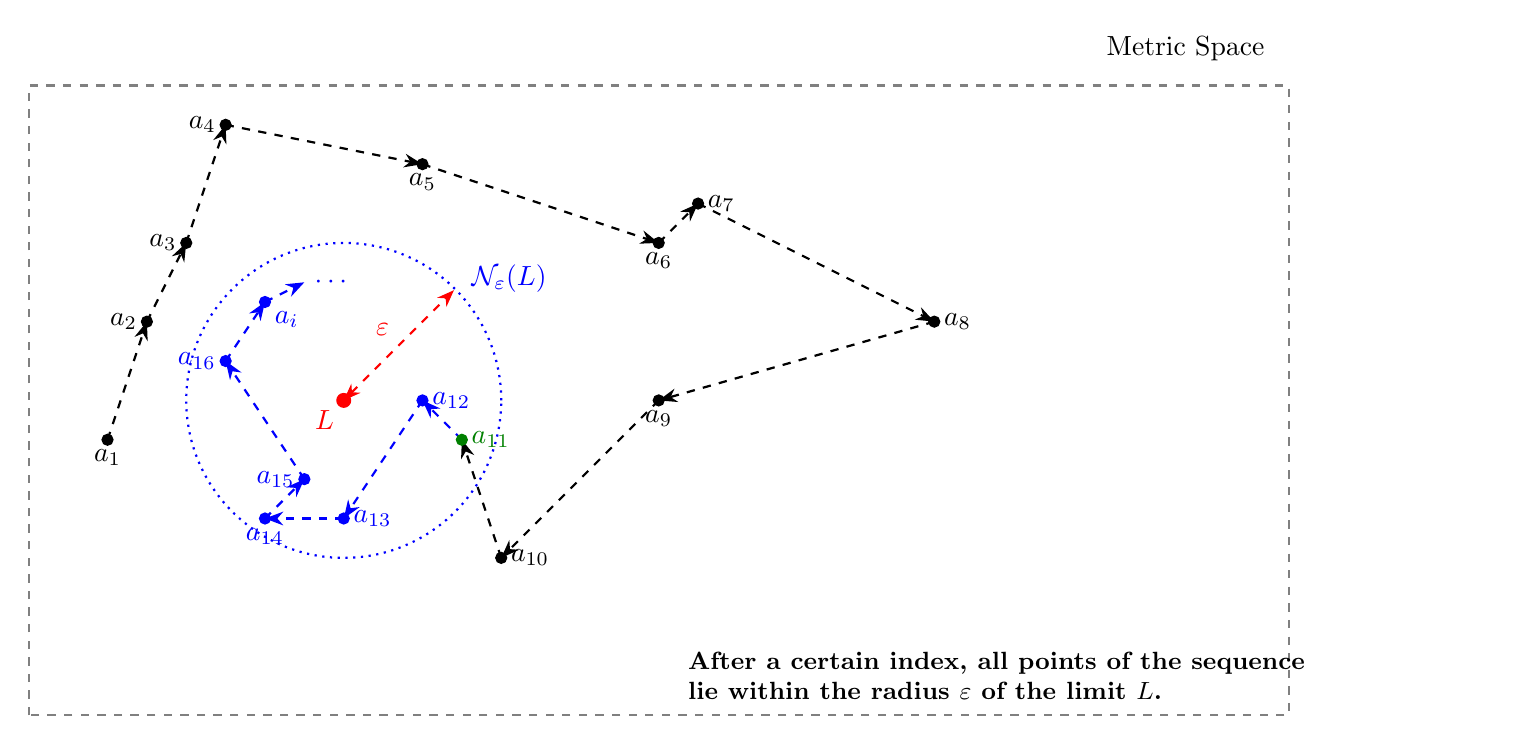
\begin{tikzpicture}[>=Stealth]
	% Draw the metric space boundary
%	\draw[thick, dashed, gray] (0,0) circle [radius=4] node[below left=3.5cm, black] {Metric Space};
	\draw[thick, dashed, gray] (-4,-4) rectangle (12,4) node[above left=.25cm, black] {Metric Space};
	
	% Mark the convergence point
	\filldraw[red] (0,0) circle (2.5pt) node[below left] {$L$};
	\draw[<->, dashed, red, line width=.25mm] (0,0) to (1.4,1.4);
	\node[above left, red] at (.7,.7) {$\varepsilon$};
	
	% Draw the epsilon neighborhood around the convergence point
	\draw[dotted, thick, blue] (0,0) circle [radius=2];
	\node[above right] at (1.5,1.25) {\textcolor{blue}{$\nbhd_\varepsilon(L)$}};
	
	% Add sequence points (outside the epsilon-neighborhood initially)
	\filldraw[black] (-3,-0.5) circle (2pt) node[below] {$a_1$};
	\filldraw[black] (-2.5,1) circle (2pt) node[left] {$a_2$};
	\filldraw[black] (-2,2) circle (2pt) node[left] {$a_3$};
	\filldraw[black] (-1.5,3.5) circle (2pt) node[left] {$a_4$};
	\filldraw[black] (1,3) circle (2pt) node[below] {$a_5$};
	\filldraw[black] (4,2) circle (2pt) node[below] {$a_6$};
	\filldraw[black] (4.5,2.5) circle (2pt) node[right] {$a_7$};
	\filldraw[black] (7.5,1) circle (2pt) node[right] {$a_8$};
	\filldraw[black] (4,0) circle (2pt) node[below] {$a_9$};
	\filldraw[black] (2,-2) circle (2pt) node[right] {$a_{10}$};
	
	% Add sequence points converging within the epsilon-neighborhood
	\filldraw[blue] (1,0) circle (2pt) node[right] {$a_{12}$};
	\filldraw[blue] (0,-1.5) circle (2pt) node[right] {$a_{13}$};
	\filldraw[blue] (-1,-1.5) circle (2pt) node[below] {$a_{14}$};
	\filldraw[blue] (-.5,-1) circle (2pt) node[left] {$a_{15}$};
	\filldraw[blue] (-1.5,.5) circle (2pt) node[left] {$a_{16}$};
	\filldraw[blue] (-1,1.25) circle (2pt) node[below right] {$a_{i}$};
	
	% Add arrows showing progression of the sequence
	\draw[dashed, ->, thick] (-3,-0.5) to (-2.5,1);
	\draw[dashed, ->, thick] (-2.5,1) -- (-2,2);
	\draw[dashed, ->, thick] (-2,2) -- (-1.5,3.5);
	\draw[dashed, ->, thick] (-1.5,3.5) -- (1,3);
	\draw[dashed, ->, thick] (1,3) -- (4,2);
	\draw[dashed, ->, thick] (4,2) -- (4.5,2.5);
	\draw[dashed, ->, thick] (4.5,2.5) -- (7.5,1);
	\draw[dashed, ->, thick] (7.5,1) -- (4,0);
	\draw[dashed, ->, thick] (4,0) -- (2,-2);
	\draw[dashed, ->, thick] (2,-2) -- (1.5,-.5);
	\draw[blue, dashed, ->, thick] (1.5,-.5) -- (1,0); % 10-11
	\draw[blue, dashed, ->, thick] (1,0) -- (0,-1.5); % 11-12
	\draw[blue, dashed, ->, thick] (0,-1.5) -- (-1,-1.5); % 12-13
	\draw[blue, dashed, ->, thick] (-1,-1.5) -- (-.5,-1); % 13-14
	\draw[blue, dashed, ->, thick] (-.5,-1) -- (-1.5,.5); % 14-15
	\draw[blue, dashed, ->, thick] (-1.5,.5) -- (-1,1.25); %16-
	\draw[blue, dashed, ->, thick] (-1,1.25) -- (-.5,1.5) node[right] {$\cdots$};
	\filldraw[green!50!black] (1.5,-.5) circle (2pt) node[right] {$a_{11}$};
	
	% Annotation for sequence behavior
	\node[right=.75cm] at (3.5,-3.5) {
		\begin{minipage}{10cm}
			\small\bfseries
			After a certain index, all points of the sequence \\
			lie within the radius $\varepsilon$ of the limit $L$.
		\end{minipage}
	};
	
\end{tikzpicture}
\end{center}	

%\begin{tikzpicture}
	
%	% Draw the metric space boundary
%	\draw[thick, dashed, gray] (0,0) circle [radius=4] node[below left=3.5cm, black] {Metric Space};
%	
%	% Mark the convergence point
%	\filldraw[red] (0,0) circle (2.5pt) node[below left] {$p$};
%	
%	% Draw the epsilon neighborhood around the convergence point
%	\draw[thick, blue] (0,0) circle [radius=2.5];
%	\node[above left=0.5cm] at (2,1.5) {\textcolor{blue}{$\nbhd_\varepsilon(p)$}};
	
	% Random sequence points
%	\pgfmathsetseed{12345} % Fix the random seed for reproducibility
%	\coordinate (prev) at (4, 0); % Initial point for the sequence
%	\foreach \i in {1,...,100} {
%		% Generate random points
%		\pgfmathsetmacro{\radius}{4 + (5 * \i / 100) + (\i > 50 ? 0.05 * (rnd - 0.5) : 0)} % Decreasing radius, within bounds after \i > 50
%		\pgfmathsetmacro{\angle}{(\i > 50 ? rnd - 2.5 : rnd * 10 - 10)} % Constrain angle tighter after \i > 50
%		\pgfmathsetmacro{\x}{\radius * cos(\angle) * 2}
%		\pgfmathsetmacro{\y}{\radius * sin(\angle) * 4}
%		
%		% Draw the point
%		\filldraw[black] (\x,\y) circle (1pt);
%		
%		% Draw a line connecting to the previous point
%		\draw[thick] (prev) -- (\x,\y);
%		
%		% Update the previous point
%		\coordinate (prev) at (\x,\y);
		
		% Label a few points
%		\ifnum\i<5
%		\node[below right] at (\x,\y) {$x_{\i}$};
%		\else\ifnum\i=50
%		\node[below right] at (\x,\y) {$x_{50}$};
%		\else\ifnum\i=100
%		\node[below right] at (\x,\y) {$x_{100}$};
%		\fi\fi\fi
%	}
	
	% Annotation for sequence behavior
%	\node[right=0.5cm] at (3,-1) {
%		\begin{minipage}{4cm}
%			\small
%			After a certain point, all dots are contained within the $\varepsilon$-radius around $p$.
%		\end{minipage}
%	};
	
%\end{tikzpicture}

\end{note}

\newpage
\defbox[Continuity of Functions]{\begin{definition*}
	Let $S\subseteq$ be a non-empty subset of $\R$. Let $f:S\to\R$ be a real-valued function, and let $a\in S$. We say that $f$ is \textbf{continuous at $a$} if and only if \[
	\lim\limits_{x\to a}f(x)=f(a).
	\] That is, \[
	\forall\varepsilon>0,\ \exists\delta>0\quad\text{such that }\quad \abs{x-a}<\delta\implies|f(x)-f(a)|<\varepsilon.
	\] If $f$ is continuous on every point of $S$, then $f$ is called a \textbf{continuous function on $S$}.
\end{definition*}}
\begin{remark*}
\ \begin{align*}
	&\forall\varepsilon>0,\ \exists\delta>0\quad\text{such that }\quad \abs{x-a}<\delta\implies|f(x)-f(a)|<\varepsilon \\
	\iff&\forall\varepsilon>0,\ \exists\delta>0\quad\text{such that }\quad x\in\nbhd_\delta(a)\implies f(x)\in\nbhd_\varepsilon(f(a))\\
	\color{gray!50}\iff&\color{gray!50}\forall\varepsilon>0,\ \exists\delta>0\quad\text{such that }\quad f(x)\in f[\nbhd_\delta(a)]\implies f(x)\in\nbhd_\varepsilon(f(a))&\color{gray!50}\because f[\nbhd_\delta(a)]=\set{f(x):x\in\nbhd_\delta(a)}\\
	\iff&\forall\varepsilon>0,\ \exists\delta>0\quad\text{such that }\quad f[\nbhd_\delta(a)]\subseteq\nbhd_\varepsilon\left(f(a)\right).
\end{align*}
\begin{center}
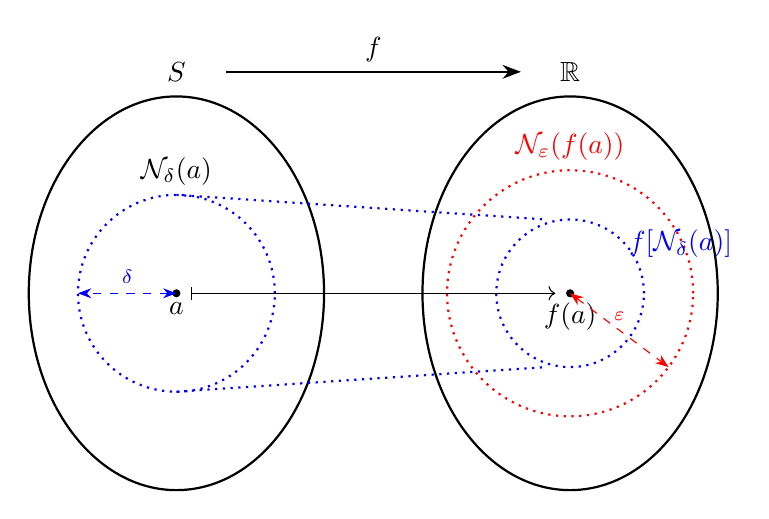
\begin{tikzpicture}[scale=1.25]
	\draw[thick] (-2,0) ellipse (1.5 and 2);
	\draw[blue, dotted, thick] (-2,0) ellipse (1 and 1);
	\node[above] at (-2,1) {$\nbhd_\delta(a)$};
	\draw[thick] (2,0) ellipse (1.5 and 2);
	\node[red, above] at (2,1.25) {$\nbhd_\varepsilon(f(a))$};
	\draw[red, dotted, thick] (2,0) ellipse (1.25 and 1.25);
	\draw[blue, dotted, thick] (2,0) ellipse (.75 and .75);
	\node[blue, right] at (2.5,.5) {$f[\nbhd_\delta (a)]$};
	
	% Labels for sets
	\node at (-2, 2.25) {$S$};
	\node at (2, 2.25) {$\R$};
	
	% Draw the arrows representing the function
	\draw[-Stealth, thick] (-1.5, 2.25) -- (1.5,2.25) node[midway, above] {$f$};
	
	%	\node at (2, 1.25) {$f[A]$};
	\draw[blue, dotted, thick] (-2, 1) -- (1.75, .75);
	\draw[blue, dotted, thick] (-2, -1) -- (1.75, -.75);
	
	\filldraw (-2,0) circle (1pt) node[below] {$a$};
	\filldraw (2,0) circle (1pt) node[below] {$f(a)$};
	\draw[|->] (-1.85, 0) -- (1.85, 0);
	
	\draw[>=Stealth, <->, dashed, red] (2, 0) -- (3,-.75) node[midway, above] {\scriptsize $\varepsilon$};
	\draw[>=Stealth, <->, dashed, blue] (-2, 0) -- (-3,0) node[midway, above] {\scriptsize $\delta$};
\end{tikzpicture}
\end{center}
\end{remark*}
\begin{remark*}
	$f$ is discontinuous at $a$ if and only if \begin{align*}
		&\exists\varepsilon>0\quad\text{such that}\quad\forall\delta>0,\ \abs{x-a}<\delta\ \text{but}\ |{f(x)-f(a)}|\geq\varepsilon\\
		\iff &\exists\varepsilon>0\quad\text{such that}\quad\forall\delta>0,\ \nbhd_\varepsilon\left(f(a)\right)\subset f\left[\nbhd_\delta(a)\right].
	\end{align*}
\end{remark*}
%\newpage
%\begin{tcolorbox}
%For a positive integer $n$, let \[
%S=\set{0,1,2,\dots, 2^n-1}=\set{\texttt{0},\texttt{01}, \texttt{10},\dots, \underbrace{\texttt{11$\cdots$ 1}}_{n\ \text{times}} }
%\] represent all integers $0$ to $2^n-1$. Define $\abs{k}$ as the Hamming weight of $k\in S$, \ie, the number of $1$'s in the binary representation of $k$. We claim that
%\begin{center}
%``For all $n\geq 1$, $\displaystyle\binom{n}{i}$ is even for $0<i<n$''.
%\end{center}
%Equivalently, \begin{center}
%``The least significant bit (LSB) of $\displaystyle\binom{n}{i}$ in its binary representation is $\texttt{0}$ for all $0<i<n$.''\end{center}
%\end{tcolorbox}
%\begin{proof}
%%The Hamming weight $\abs{k}$ of $k\in S$ is defined as \[
%%\abs{k}=\sum_{i=0}^{n-1}b_i,\quad b_i\in\set{0,1}.
%%\]
%The binomial coefficient $\binom{n}{i}$ is defined as: \[
%\binom{n}{i}=\frac{n!}{i!(n-i)!}.
%\] For any positive integer 
%$k$, the number of factors of 2 in $k!$, is given by:
%$$\sum_{j\geq 1}\floor*{\frac{k}{2^j}},$$
%where $\floor*{\frac{k}{2^j}}$ counts how many multiples of $2^j$ appear in $k$. For example, $5!=$
%\end{proof}

\newpage
\begin{note}
	TBA
\end{note}
\begin{note}
	TBA
\end{note}
\vfill

\begin{thebibliography}{9}
	\bibitem{advanced_topo_a}
	수학의 즐거움, Enjoying Math. ``수학 공부, 기초부터 대학원 수학까지, 8. 위상수학 (a) 위상공간의 정의.'' YouTube Video, 41:25. Published 
	September 27, 2019. URL: \url{https://www.youtube.com/watch?v=q8BtXIFzo2Q}.
	\bibitem{advanced_topo_b}
	수학의 즐거움, Enjoying Math. ``수학 공부, 기초부터 대학원 수학까지, 9. 위상수학 (b) 해석학개론과 거리위상'' YouTube Video, 33:43. Published 
	September 29, 2019. URL: \url{https://www.youtube.com/watch?v=uJOGw7Yxk7c&t=242s}.
\end{thebibliography}
%\newpage
%\appendix
%\section{Complement of Family}
%\begin{note}
%	\[
%	\left(\bigcup_{i\in\Lambda}E_i\right)^C=
%	\bigcap_{i\in\Lambda}\left(E_i\right)^C
%	\]
%	\begin{proof}
%		content...
%	\end{proof}
%\end{note}
\end{document}
